\section{Datasets}

%%%%%%%%%%%%%%%%%%%%%%%% Bias
\section{Bias}
\label{sec:data_bias_overview}

\subsection{Types of Bias}

\subsubsection{Interaction Bias}

\subsubsection{Latent Bias}

\subsubsection{Selection Bias}

\subsubsection{Recency Bias}

\subsection{Evaluation}

\textcolor{blue}{Performance evaluation on subsets of your data}

\textcolor{blue}{Evaluating false positives and false negatives for these subsets in the context of the problem/application.}

\textcolor{blue}{Equality of Opportunity -- gives individuals an equal chance}


%%%%%%%%%%%%%%%%%%%%%%%% Acquiring Data
\section{Data Acquisition}


\subsection{Resources}

\subsection{Generating Fake Data}

\textcolor{green}{TODO: generating fake data with SKL}

\textcolor{blue}{make\_blobs}

% {{{datagen_blobs_2dcode}}}
\begin{lstlisting}[style=pyInStyle]
X, y = datagen.make_blobs(centers=4, n_samples=100, n_features=2,cluster_std=1.0,
                          center_box=(-10, 10),
                          random_state=42, shuffle=True)
\end{lstlisting}

% {{{datagen_blobs_2dimg}}}
\begin{figure}
\centering
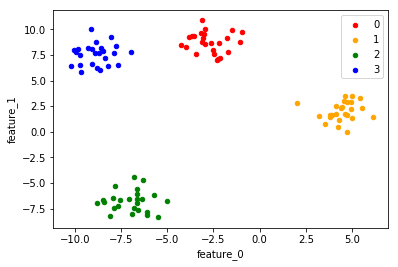
\includegraphics[width=0.65\textwidth]{./sync_imgs/datagen/blobs/2dimg.png}
\label{fig:datagen_blobs_2dimg}
\end{figure}

\textcolor{blue}{Data can also be generated in three (multiple) dimensions}

% {{{datagen_blobs_3dcode}}}
\begin{lstlisting}[style=pyInStyle]
X, y = datagen.make_blobs(centers=4, n_samples=100, n_features=3, random_state=42)
\end{lstlisting}

% {{{datagen_blobs_3dimg}}}
\begin{figure}
\centering
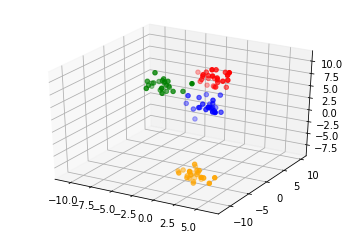
\includegraphics[width=0.65\textwidth]{./sync_imgs/datagen/blobs/3dimg.png}
\label{fig:datagen_blobs_3dimg}
\end{figure}

%\textcolor{blue}{More dataset types can be generated, the documentation can be found at (http://scikit-learn.org/stable/modules/classes.html#module-sklearn.datasets)}


\textcolor{blue}{see \textcolor{red}{local ref?} for more examples on how to generate data}


%%%%%%%%%%%%%%%%%%%%%%%% Data Pre-processing
\section{Data Preparation}

\textcolor{blue}{TODO: direct and indirect importance of datapreparation. indirect: feature engineering allows for more elegant and efficient solutions (e.g. calculating the time with a CNN of a clock face vs engineered features for the angles of the large and small hand.) }

\subsection{Data Pre-processing}

\textcolor{blue}{Data is rarely obtained in a form that is necessary for optimal performance of a learning algorithm. Data can be missing, can contain a mix of categorical and quantitative, can contain values on vastly different scales, etc.}

\textcolor{blue}{Building a good representation of your data -- feature extraction/engineering}

\textcolor{blue}{It is important to note that any parameters related to data pre-processing, such as feature scaling and dimensionality reduction, are obtained solely from observing the training set. The parameters for these methods obtained on the training set are then later applied to the test set. This is important since if these preprocessing parameters were obtained on the entire dataset and included the test set, the the model performance may be overoptimistic since then when applying the methods to the unseen data.}

\textcolor{blue}{make sure to use data that is relevant to the objective/problem.}

% TODO: case study example

\textcolor{blue}{make sure the data can be known at prediction time. e.g. will there be a delay between activity and being able to access that data at the data repository?}

% TODO: case study example

% TODO: expand
\textcolor{blue}{features should be numeric and have a meaningful magnitude (see below). In addition to being meaningful, the magnitude should be on a similar (small) range. e.g. if some data has one feature on a range 70,000-500,000 (estimated home value) and another feature on a 0-5 range (maybe number of bathrooms in a house), the higher values, in addition to being viewed as more meaningful (higher weights), large gradient updates may result that don't allow the network to converge (the updates are not fine grained enough).}

% TODO: case study example

\r{pre-processing may be used to reduce the dimensionality of the data, before training.}

\textcolor{blue}{make sure ``enough'' examples exist for the particular feature}

\textcolor{blue}{Don't mix magic values with values you already have. For example, if we have ratings 0-10, don't include a new column for rated vs not rated.}

\subsubsection{Handling Missing Data}

\paragraph{Filtering Out}

\textcolor{blue}{Simply removing any entries that are missing data. This is convenient and easy but may not be practical -- any time data is being removed, potentially useful information is lost and too much data may be removed.}

\textcolor{green}{TODO: Code in jupyter on how to do this with pandas and dropna -- key params - how, thresh, subset}

\paragraph{Filling In}

\textcolor{blue}{Estimating the missing data}

\subsubsection{Handling Categorical Data}

\paragraph{Encoding}

\textcolor{blue}{It may seem intuitive to represent categorical data with an integer value. However, this may not always be best. Let's pretend we're representing United States with arbitrary integer values and we assign values alphabetically; Alabama: 0, Alaska: 1, Arizona: 2, Arkansas: 3, California: 4, ..., Wisconsin: 48, Wyoming: 49. So far so good. \textcolor{red}{However, these values indirectly imply a relationship (that may not actually exist)} -- and imply that some states are more similar to one another than others (for instance, this encoding seemingly indicates that Alabama as most related to Alaska.) }

\textcolor{blue}{{one-hot encoding}\index{one-hot encoding} or one-of-k encoding\index{one-of-k encoding} is a method of encoding which represents each explanatory variable as a binary feature}

\textcolor{blue}{one-hot encoding reduces the relationship}

\textcolor{green}{TODO: show example of one hot encoding}

\textcolor{blue}{will lead to {sparse vectors}\index{sparse vectors} -- high dimensional vectors. This is memory intensive (some libraries have methods to address this --- SciPy and Pandas).}

\subsubsection{Feature Scaling, Normalization}

% TODO: this section needs to be restructured to present ideas in a logical flow/building on one another and the cost(time)/benefit

\textcolor{blue}{Ensuring variables exist on a similar scale and variance is important. If one variable is orders of magnitude larger than others, the variable may dominate the learning algorithm and prevent influence from the other variables.}

\textcolor{blue}{Generally would like to get each feature into the $-1 \le X_i \le 1$ or the $-0.5 \le X_i le 0.5$ range.}

\textcolor{blue}{"OK" if not exact, different people have different rules of thumb for when it is necessary to scale a feature into this range.}

\textcolor{blue}{Additionally, some learning algorithms converge more slowly.}

% hard clipping/capping

% log scalling -- good for when the data has a huge range

% TODO: Give an example


\paragraph{Mean Normalization}

\textcolor{blue}{feature $x$ is replaced by $x - \mu$ to create a zero mean}

% TODO: 2D figure showing a circle vs oval contour plot and how gradient descent may take longer on the "oval"

\paragraph{Min-Max scaling (Normalization)}

\textcolor{blue}{values are shifted and rescaled so they end up on a [0,1] range}

\paragraph{Standardization}

\textcolor{blue}{(Eq.~\ref{eq:preprocess_standardization}) first, subtract the sample mean, then divide by standard deviation variance}

\textcolor{blue}{pros: unlike min-max, not bound to specific range}

\textcolor{blue}{standardized values always have a zero mean and unit variance, a standard deviation of 1.}

\textcolor{blue}{gives our data the property of a standard normal distribution}

\begin{equation}
{X' = \frac{X - \mu}{\sigma}}
\label{eq:preprocess_standardization}
\end{equation}

\textcolor{green}{TODO: create code sample - numpy, and sklearn methods}

\subparagraph{Robust Scaler}

\textcolor{blue}{In order to reduce the effect of large outliers, a \textcolor{blue}{RobustScalar} may be used. Rather than subtract the mean and divide by the standard deviation, the median is subtracted and then the data is divided by the {interquartile range}\index{interquartile range} -- \textcolor{red}{see local ref?}}


\subsubsection{Others}

\paragraph{Removing Duplicates}

\paragraph{Outliers}

\textcolor{blue}{rather than remove outliers, the values may be capped.}
% TODO: example, in the California housing data, there are datapoints with 50 rooms per house

\paragraph{Discretization and Binning}

\textcolor{blue}{An example for this may be housing prices and latitude.}

% ? tf.feature_column.bucketized_column

\textcolor{blue}{rather than store a floating point, bins could be created. would like to keep the information (latitude may be useful, but the magnitude here is not useful (even if normalized) and so binning may be a great option)}

% TODO: figure for latitude (housing prices) and values pre/post binning

\subsubsection{Where to do preprocessing}

\textcolor{blue}{1. at execution time/with the TF graph}
\textcolor{blue}{2. apache beam ``in front'' of the graph (can use time windows)}
\textcolor{blue}{3. }



\textcolor{blue}{Batch vs Streaming}

% calculating rolling average

\subsubsection{Feature Engineering}

\textcolor{blue}{feature engineering is the process of altering the values of the data such that the problem becomes easier to solve as a result of expressing the data in a simplier/more relevant way. this usually required domain knowledge.}

\textcolor{green}{TODO: p.102 of Keras book fchollete uses a clock example that is very nice.}

%%%%%%%%%%%%%%%%%%%%%%%% Data Type Considerations + Feature Extraction
\section{Feature Extraction from Various Datatypes}

\textcolor{green}{TODO: Feature Extraction}


\subsection{Images}

\textcolor{green}{TODO: Images}


\subsubsection{Video}

\textcolor{green}{TODO: Video}


\subsection{Natural Language}

\textcolor{green}{TODO: Natural Language}

\subsubsection{Terminology}

\textcolor{blue}{A {corpus}\index{corpus} is a collection of documents. {vocabulary}\index{vocabulary} is a corpus's unique words}

\subsubsection{Pre-processing}

\textcolor{green}{TODO: Pre-processing}

\textcolor{blue}{converting all letters to lowercase}

\textcolor{blue}{stemming and lemmatization --- Condensing word forms (derived and inflected) into a single feature. These methods are used to reduce the dimensionality of the features space.}

\paragraph{Stop Word Filtering}

\textcolor{blue}{todo: removing words that are common throughout the language as well as potentially to most of the documents in a corpus. Typically stop words do not convey meaning through their meaning, but rather through their grammatical meaning.}

\paragraph{Tokenization}

\textcolor{blue}{Tokenization is the process of splitting and grouping characters together into meaningful sequences. \textcolor{red}{If a document is tokenized, the result is a set of tokens (words).} Tokens are not limited to words however, and may also be shorter sequences like punctuation characters and affixes.}

\textcolor{green}{TODO: Tokenization example}

\paragraph{Lemmatization}

\textcolor{green}{TODO: Lemmatization. converting words into their base form --- determining the lemma (morphological root) of an inflected word.}

\paragraph{Stemming}

\textcolor{green}{TODO: Stemming. There exist many stemming algorithms. Stemming removes all character patterns that appear to be affixes to a word. Note: the resulting word may or may not be a valid word e.g. \textcolor{red}{XXXXXXXX}.}

\subparagraph{Porter Stemming}

\subsubsection{Encoding}

\paragraph{Encoding Methods}

\subparagraph{Bag-of-Words}

\textcolor{blue}{{bag-of-words}\index{bag-of-words} similar to one-hot-encoding, it encodes words that appear in text as one feature for each word of interest. Does not encode any other information like syntax, grammar, or order of the words.}

\textcolor{blue}{Bag-of-Words encodes the corpus's vocabulary as a feature vector to represent each document. The intuition for using bag-of-words is that documents that contain similar words are likely to be similar to one another.}


\paragraph{tf-idf}

\textcolor{green}{TODO: tf-idf\index{tf-idf} (Eq.\ref{eq:tf_idf_def}) Inverse Document Frequency is a measure of how common/rare a term is in a corpus --- explain importance}

\begin{equation}
{log\frac{N}{1|XXXXXXXXTODOXXXXXXXXXX|}}
\label{eq:tf_idf_def}
\end{equation}

\subsubsection{Embedding}

\subparagraph{glove}

\textcolor{green}{TODO: glove}

\subparagraph{word2vec}

\textcolor{green}{TODO: word2vec}

\subsubsection{Other Notes}

% 'hashing trick' --- see p59 of Mastering ML with SKL

\subsection{Audio}


\textcolor{green}{TODO: Audio}



%%%%%%%%%%%%%%%%%%%%%%%% Data sampling and partitioning
\section{Partitioning Data}

\textcolor{blue}{Ideally, a model will generalize well i.e. a model will perform well on data that it has never seen. When evaluating a model, the performance is reported on a data that has never been seen by the model. When a dataset is obtained, one of the first steps performed is to partition the dataset -- a portion of the dataset is removed and placed aside as the ``test'' set that will later be used to measure the performance of an indicated model.}

\subsection{Types of Splits}

\textcolor{blue}{A learning method is trained on a collection of examples called the ``training set''. The performance of the learning method is then evaluated on another collection of examples known as the ``test set''. It is important to ensure that none of the instances in the test set are included in the training set -- a point that will be mentioned many times throughout this text. If the test set were to include examples from the training set, evaluating the whether the learning method has memorized the training set or generalizes well will be difficult.}

\textcolor{blue}{An additional set, known as the validation is typically used. The validation set is used to tune the hyperparameters of the learning algorithm and help prevent overfitting to the training data. Though the model does not train directly on the validation dataset (exception being when using k-folds cross validation) it is still possible to overfit the validation set since we are manually adjusting the hyperparameters to give the best result on the validation set. This situation is related to the concept of {information leaks}\index{information leaks} --- some information from the validation data \textit{leaks} into the model by tuning hyperparameters with regard to this information. This will generally lead to a  model that performs artificially well on the validation set (since this is what was optimized for)}

\textcolor{blue}{Along these same lines, it should be noted that evaluating on the test set should only be performed \textbf{once}.\textcolor{red}{this is important}. Otherwise, the model will be tuned to the test set, resulting in overly optimistic results. To compare different design choices to one another, it is best to compare and finalize them based on their performance on the validation set, before ``locking'' the model and evaluating its performance on test set.}

\begin{figure}[htp]
	\centering
	\includegraphics[width=0.5\textwidth]{example-image-a}\hfil
	\caption{Figure showing when to save best parameters (plus link to ``early stopping''), \textcolor{green}{TODO}}
	\label{fig:sample_split_save_best_params}
\end{figure}

\textcolor{blue}{There are no hard rules that clearly define how a dataset should be divided into training, validation, and test sets and usually the ratio of data in each split depends on the overall size of the dataset.}

\textcolor{blue}{Some common dataset splits (training:validation:test) are 50:20:30 and 40:20:40}

\begin{figure}[htp]
	\centering
	\includegraphics[width=0.5\textwidth]{example-image-b}\hfil
	\caption{Figure showing hold and common dataset splits, \textcolor{green}{TODO}}
	\label{fig:sample_split_hold_out}
\end{figure}

\textcolor{blue}{``hold out'' split}

\textcolor{blue}{{lucky split}\index{lucky split} is used to describe an instance in which, by chance, the test set contains easily predicted instances and the training set includes difficult to predict instances.}

\textcolor{blue}{Typically the performance of a machine learning algorithm improves with the number of training instances. However, quality is superior to quantity, in that a lot of ``bad'' data is worse than a smaller amount of ``good'' data -- in this sense, machine learning algorithms follow the ``garbage in, garbage out''.}



\subsection{k-Fold Cross Validation}

\r{cross validation is a method used to train across the entire training dataset without holding out an explicit validation set. The training data is partitioned, into $k$ ``folds'', and the algorithm is trained on all but one of these partitions and evaluated on the remaining partition. The partitions are then rotated such that each fold/partition is included in the training and evaluation of the algorithm. After sufficient training, (as defined by the individual), the model is then evaluated on the test set.}

\TD{stratfied k-fold cross validation}

\begin{figure}[htp]
	\centering
	\includegraphics[width=0.5\textwidth]{example-image-a}\hfil
	\caption{Figure showing how k-fold cross validation works, \textcolor{green}{TODO}}
	\label{fig:sample_split_k_fold}
\end{figure}

\subsubsection{k-Fold Validation with shuffling}

\textcolor{blue}{shuffle the data before splitting it k-ways --- where k-fold validation is performed multiple times}

% TODO: design a warn/caution/watch-out box
\textcolor{green}{WARN: every time you fold in the data/train on the data, the ``information leak'' is greater -- leading to likely overfitting}

\subsection{Sampling}

\textcolor{blue}{Things to consider when performing splits. How representative your data is -- compared to the population and compared to each split.}

\paragraph{Representative Data}

\begin{figure}[htp]
	\centering
	\includegraphics[width=0.5\textwidth]{example-image-b}\hfil
	\caption{Figure showing importance of shuffling data. one figure where the data isn't shuffled well and a split leads to a case where one split contains only a subset of the classes (not all the classes) \textcolor{green}{TODO}}
	\label{fig:sample_split_shuffle_importance}
\end{figure}

\textcolor{blue}{NOTE/WARN: only perform shuffling when it makes sense --- e.g. shuffling time series data would not be wise.}

\textcolor{blue}{WARN: It would be smart to check your data for any points where the same instance is included across both splits training/validation/test. If the dataset contains multiple samples of the same instance, and they are inluded in different splits, there is now redundancy and even worse: imagine a situation in which the same instance (e.g. the same image or an image of the same object, just at a different angle) we now are training on our test set!  Bottom line: it is important to ensure the training, validation, and test sets are all disjoint.}

\paragraph{Representative Data}

\textcolor{blue}{Random vs \textcolor{red}{stratified}}

\TD{Stratified -- preserves ratio}


\subsection{Transform}

\subsubsection{Overview}

\textcolor{blue}{TensorFlow Transform is a library used for preprocessing data with TensorFlow.}

\textcolor{blue}{MOTIVE: calculating values (such as $\mu$ and $\sigma$) for an entire dataset can be challenging for large datasets.}

\textcolor{blue}{Though preprocessing can already be accomplished with standard python, numpy, other libraries, or even in TensorFlow, tf.Transform extends these capabilities to support full passes over the dataset.}

\subsubsection{Installation}

\textcolor{green}{TODO: include snippet for installation}

\subsubsection{Implementation}

\textcolor{green}{TODO: include use examples}
% https://github.com/tensorflow/transform/blob/master/getting_started.md


% resources
% 1. https://github.com/tensorflow/transform
% 2. https://github.com/tensorflow/transform/blob/master/getting_started.md


\section{Building Architectures}

\subsection{Layers}

\subsection{Estimators}

% TODO: entire section

% boilerplate code
% graph and session management
%\textcolor{blue}{}
% distribute training and evaluation of a model

\subsubsection{Input data}

% TODO: input function overview

\paragraph{Specifying Hyper Parameters}

\subparagraph{Epochs}
\textcolor{blue}{by default, training will continue until the training data is exhausted, or the number of specified epochs is reached}

Options:

%TODO: code example
\begin{enumerate}
	\item input\_fn
	\item steps
	\item max\_steps --- will potentially do nothing if the checkpoint has already reached this value
\end{enumerate}


\paragraph{In Memory Data}

\textcolor{blue}{Usually this is in the form of either numpy arrays or pandas dataframes. These can both be used directly.}

% TODO: examples for Numpy array

% TODO: examples for Pandas DF

\paragraph{Out of Memory Data}

\textcolor{blue}{In the ``real world'' the dataset will likely not fit into memory. To (sanely) address this, estimators play nicely with the tf.Data API (please see \textcolor{red}{local ref} for more information)}

% TODO: show quick demo example

% tf.estimator base class allows you to build your own model 

% premade models (TODO: Show quick list)

% main advantage -- estimators are interchangable

% "reasonable" defaults for each estimator

\subsubsection{Checkpoints}

\textcolor{blue}{directory specified when creating model. By default, predictions will be made from the latest checkpoints in this directory. training also resumes from the latest checkpoint in the directory. --- to start from scratch, the directory will need to be deleted or specified to a new location.}

\subsubsection{Distributed}

% you need: 1. estimator, 2. run config, 3. train spec, eval spec

% final call tf.estimator.train_and_evaluate(estimator, train_spec, eval_spec)

\paragraph{tf.estimator.RunConfig}

% TODO: example

\textcolor{blue}{the directory for checkpoints and Tensorboard logs and freq of checkpoints (save\_checkpoint\_steps) and frequency of logs (save\_summary\_steps)  }

\paragraph{tf.estimator.TrainSpec}

\textcolor{blue}{pass in input function (likely through data API (see \textcolor{red}{localref})), }


\paragraph{tf.estimator.EvalSpec}

\textcolor{blue}{pass in input function for evaluation dataset (likely through data API (see \textcolor{red}{local ref})),}

\textcolor{blue}{creates model and loads latest checkpoint, then runs eval. Therefore, you cannot get a frequency greater than the checkpoints created. They can be obtained less frequently by using the `throttle\_specs` parameter}

\paragraph{Notes}

\textcolor{blue}{Shuffling considerations.use the dataset = tf.data.Dataset().list\_files().shuffle() command --- each worker a different seed? Even if the data is shuffled on disk. Can also use the dataset().shuffle()}

\subsubsection{TensorBoard}

% TODO: example -- to create: tf.estimator.RunConfig(model_dir='some_dif')

\textcolor{blue}{to visualize, then open tensorboard by issuing `tensorboard --logdir output\_dir` and the dashboard will appear on localhost:6006}

\textcolor{blue}{pre-made estimators already export relevant metrics, embeddings, histograms, etc.. for more information on how to use tensorboard please see \textcolor{red}{local ref}}

\textcolor{blue}{if building a custom estimator or would like to add additional information to tensorboard, summaries can be added with any of the following: tf.summary.scalar, tf.summary.image, tf.summary.audio, tf.summary.text, tf.summary.histogram}

\paragraph{Adding Custom}

% tf.summary.scalar('meanVar_01', tf.reduce_mean(var_01))

\subparagraph{tf.summary.scalar}

\subparagraph{tf.summary.image}

\subparagraph{tf.summary.audio}

\subparagraph{tf.summary.text}

\subparagraph{tf.summary.histogram}


\subsubsection{Deployment}

% TODO: examples

%\textcolor{blue}{two things 1) export\_latest = tf.estimator.LatestExporter(serving\_input\_receiver\_fn=serving\_input\_fn) and then eval_spec = tf.estimator.EvalSpec(input\_fn=eval\_input\_fn, exporters=export\_latest)}

% will map from JSON from REST API and the model

% important to use tf commands in the input transformation/parsing function

\paragraph{Exporters}

\textcolor{blue}{there are many types of exporters and exporter schemes. The simplest may be the tf.estimator.LatestExporter}




\subsection{Eager}


\section{Design and Component Considerations}

\subsection{Initialization Strategies}

\textcolor{blue}{Discuss different initialization strategies and their importance}

\textcolor{blue}{truncated normal -- truncated Gaussian distribution}

\subsection{Hyperparameters}

\subsubsection{Training Related}

\paragraph{Learning Rate}

\subparagraph{Too High vs Too Low}

\textcolor{blue}{TODO: figure showing a convex cost function and the result of a learning rate being too high (overshoot, diverge) and too small (local minima)}

\paragraph{Batch Size}

\paragraph{Number of Training Iterations}

\paragraph{Momentum}

\paragraph{Weight Update}

\textcolor{red}{SGD, CG, L-BFGS, more complex more hyper-parameters}

\paragraph{Stopping Criteria}

\subsubsection{Model Related}

\paragraph{Architecture}

\paragraph{Weight Initialization}

\paragraph{Weight-decay}

L1

L2

\paragraph{Drop-out}



\subsection{Hyper-parameter optimization}

\textcolor{blue}{OVERVIEW}

\subsubsection{Coordinate Descent}

All hyper-parameters remain fixed, except for the hyper-parameter of interest. The hyper-parameter of interest is then adjusted such that the validation error is minimized.

\subsubsection{Grid Search}

\textcolor{green}{TODO: grid search explanation}

\subsubsection{Random Search}

\textcolor{green}{TODO: random search explanation}

\subsubsection{Grid vs Random Search}

\textcolor{green}{TODO: grid vs random search figure}

\subsubsection{Automated / Model-based Methods}

\subsection{Optimizers}

\textcolor{blue}{Estimate the values of the model's parameters that minimize the value of the cost function}

\textcolor{blue}{"turning a loss function into a search strategy"}

\subsubsection{Gradient Descent}

\textcolor{blue}{Gradient Descent --- overview --- optimization algorithm that can be used to estimate the local minimum of a function}

\textcolor{blue}{Iteratively updates the model parameters by calculating the partial derivatives of the cost function at each step during training}

\textcolor{blue}{Gradient descent is only guaranteed to find the local minimum of the cost function.}

\textcolor{blue}{simultaneous update.}


\paragraph{Batch Gradient Descent}

\textcolor{blue}{batch gradient descent --- taking a step (update the weights) opposite (down) the gradient calculated from the entire training set}

\textcolor{blue}{Batch gradient descent is deterministic --- will produce the same paramter values if the same dataset is used multiple times.}


\paragraph{Stochastic Gradient Descent}

\textcolor{blue}{Stochastic Gradient Descent (sometimes called iterative or on-line gradient descent) --- rather than update the weights based on the sum of the accumulated errors, the weights are updated for each training sample}

\textcolor{blue}{Stochastic gradient descent is deterministic --- may produce the different parameter values if the same dataset is used multiple times. May not minimize the cost function as well as gradient descent but the approximation is often ``close enough''.}


\paragraph{Mini-batch Gradient Descent}

\textcolor{blue}{mini-batch gradient descent --- compromise between batch and stochastic gradient descent where the gradient is calculated over a batch of training data}

\textcolor{blue}{Since the gradient is calculated on a single example, the error surface will appear noisier than if it was calculated over a batch or the entire training set.}

\textcolor{blue}{When using stochastic gradient descent, it is important to shuffle the data after each epoch.}


% when looking at specific optimizers, http://ruder.io/optimizing-gradient-descent/ was a useful resource

\subsection{Improved Optimizers}

\textcolor{blue}{Some of the common optimizers are listed below. Additional optimizers are discussed in \textcolor{red}{local ref?}}

\subsubsection{Momentum}

\textcolor{blue}{Momentum~\cite{qian1999momentum}, will reduce the learning rate when the gradient is small}

\subsubsection{RMSProp}

\subsubsection{Nesterov}

\textcolor{blue}{Nesterov accelerated gradient (NAG)}

\subsubsection{Adam}

\textcolor{blue}{Adaptive Moment Estimation (Adam)~\cite{kingma2014adam}}


%%%%%%%%%%%%%%%%%%%%%%%%%%%%%%%%%%%%%%%%%%%%%%%%%%%%%%%%%%%%%%%%%%%%%%%%%%%%%%%%%%%%%%
%%%%%% TODO: Cut off -- these optimizers will be moved to another location (research?)
%%%%%%%%%%%%%%%%%%%%%%%%%%%%%%%%%%%%%%%%%%%%%%%%%%%%%%%%%%%%%%%%%%%%%%%%%%%%%%%%%%%%%%

\subsubsection{Nadam}

\textcolor{blue}{Nadam (Nesterov-accelerated Adaptive Moment Estimation)~\cite{dozat2016incorporating}}

\subsubsection{AdaGrad}

\textcolor{blue}{Adagrad~\cite{duchi2011adaptive}, will assign frequently occurring features low learning rates}

\subsubsection{AdaDelta}

\textcolor{blue}{Adadelta~\cite{zeiler2012adadelta}, expands on AdaGrad by avoiding reducing the learning rate to zero.}

\subsubsection{AdaMax}

\subsubsection{Ftrl}

\textcolor{blue}{``follow the regularized leader'', \textcolor{red}{CITE}, \textcolor{red}{works well on wide modes?}}







\chapter{Improving Generalizability}

\r{The methods shown in the upcoming sections aim to reduce overfitting. That is, these methods aim to prevent the model from becoming too specialized to the training dataset in hopes that it will generalize to data that it has not specifically seen. It is worth noting that by implementing some of these methods (e.g. reducing the model capacity), the model often has less ability to model the training set as well as it might otherwise be able to. This is ok, but worth remembering such that some of the methods aren't used before they are necessary \TD{section on determining overfitting}.}

% TODO: index overfitting
\r{overfitting: a practical definition may include observing the training loss to improve while the validation loss degrades. \TD{possibly mention \\cite{Nakkiran2020DeepDD}}}

\r{Overfitting --- too complex --- Occam's razor --- hypothesis with the fewest assumptions is best}

\r{A specific instance of improving generalization might be accounting for imblance. Either in the labels or in the features.  Section \ref{app_data_imbalance} discusses this topic and strategies in more detail.}

\r{Typicaly types of modifications that are made to improve generalization.}

\begin{itemize}[noitemsep,topsep=0pt]
	\item Data
	\begin{itemize}[noitemsep,topsep=0pt]
		\item Increase ammount of data
		\item Augmentation
		\item Sampling
	\end{itemize}
	\item Architecture --- Reduce complexity of model e.g. applying parameter constraints, and/or reduce overall number of parameters
	\begin{itemize}[noitemsep,topsep=0pt]
		\item Reduce complexity/number of parameters
		\item Ensembling
		\item Constraints
		\begin{itemize}[noitemsep,topsep=0pt]
			\item Directly on parameters
			\item Through additional losses/tasks
		\end{itemize}
	\end{itemize}
	\item Training Pattern
	\begin{itemize}[noitemsep,topsep=0pt]
		\item Early stopping
		\item Stochastic Behavior
	\end{itemize}
\end{itemize}


\section{Data}

\subsection{Data Collection}

\r{Arguably the best way to increase generalizability of a model is to train the model on more data. However, as readers may already be aware, this is not always easy. Collecting more data may not be time/cost effective, or even possible.}

\r{``free'' data in that the ``cost'' is minor computation}

\subsection{Augmentation}

\r{Dataset augmentation is \textcolor{green}{TODO}}

\r{Please note, augmentation must be done responsibly. For example, if performing digit recognition, it would not be wise to perform rotational or flip transformations on the data since, depending on the specific data, a 6, rotated 180 or flipped vertically may now appear as a 9.}


\r{invariances in the data}

\r{For specific techniques, see~\ref{app_aug_techniques}}

\TD{Beyond improving generalization, augmentation may be used in other contexts as well, such as in helping quantify uncertainty -- \TD{see ref ---\TD{Augmenting the test set. A simple augmentation (horizontal filliping) was performed on the test set in \cite{simonyan2014very} -- where the prediction of the original and augmented images are averaged to obtain the final output score.} }}


\subsection{Sampling}

\r{The line between the techniques described here and ``augmentation'' might be a little blurred, in that sampling might technically be considered a augmentation technique (and I'm not even sure ``sampling'' is the appropriate title). But the intended distinction is that in augmentation, we are diliberately altering something (e.g. the input data) and in sampling, we are altering the number of times an architecture sees a particular instance in a training dataset.}



\section{Architecture}

\section{Training Pattern}

\subsection{Early Stopping}

\r{see p.243 of DL, papers Bishop 1995 and Sjoberg and Ljung 1995}

% TODO: note about regularization --- the smaller the value, the stronger the regularization.


\subsection{Stochastic Behavior}

\subsubsection{Dropout}

\r{``Dropout'' as a node in a computational graph may be considered an architectural structure change, but the method itself affects the training pattern in possibly not obvious ways. }

% TODO: explain dropout

\r{Dropout -- ref original paper (Hinton? -- intuitive, inspired by bank -- that defrauding the bank would require cooperation between employees to defraud the bank \TD{cite})}.

\r{Dropout (proposed in ``Improving Neural Networks by Preventing Co-Adaption of Feature Dectors''~\cite{DBLP:journals/corr/abs-1207-0580}, and popularized by Nitish et.al in ``Dropout: a Simple Way to Prevent Nerual Networks from Overfitting''~\cite{JMLR:v15:srivastava14a}}

\r{It is important to note that dropout is only present during training. i.e. dropout does not occur during test/evaluation if using dropout in the ``standard way''. However dropout is occassionally used for evaluation in attempt to quantify model uncertainty \TD{CITATION}}

\r{keeps a neuron active by a hyperparameterized probability.}

\r{used in any/all neurons in the network (other than the output neruons).}

\r{think about where dropout is used. That is when you use dropout at any given nueron the upstream paths transversing that particular neuron are also affected (in this case, ``turned off''), as well downstream connections (but often only modified, not entirely turned off since they often still have other inputs) }

\r{Forces the network to learn mappings even in the absence of all the information, that is the network is forced to consider the values of other values and can't rely on a smaller number of values or groups of values. Said another way, the network is prevented from becoming too dependent on certain inputs or features.}

\r{In this way, dropout can be thought of as sort of an ensembling method. When dropout is in use during training, each loop technically produces a different network that is then trained for the given task. During the next loop, a different network is used. As Aurélien Géron~\cite{geron2019hands} describes, if you train for 10,000 training steps (where dropout is used), you will have likely (almost certainly) trained 10,000 different neural networks. It's true that each network is not indpendant (they share weights), but they are different. More generally, a network with $N$ activations with dropout present, there exist $2^N$ possible networks ($2$ since each activation/neuron/value can have either an `on` or `off` state.) and thus, the use of all of these networks at once can be considered an ensembling of sorts.}

\TD{create figure of this ensemble of many networks.}


% TODO: find recent paper I saw mentioned on twitter.... (4July) it may be in my pocket

\begin{figure}[htp]
	\centering
	\includegraphics[width=0.3\textwidth]{example-image-a}\hfil
	\includegraphics[width=0.3\textwidth]{example-image-b}\hfil
	\includegraphics[width=0.3\textwidth]{example-image-c}\hfil
	\caption{\TD{Graph of an example function including dropout. three separate training iterations and how the network changes}}
	\label{fig:regularization_dropout_overview_training}
\end{figure}

\begin{figure}[htp]
	\centering
	\includegraphics[width=0.3\textwidth]{example-image-a}\hfil
	\caption{\TD{Same graph during test --- no dropout applied}}
	\label{fig:regularization_dropout_overview_test}
\end{figure}

\r{It is worth pointing out that since dropout is only applied at training time, comparing the loss curve of training and inference (validation splits) will be a bit misleading since the full ensemble network is used for calculating the validation loss/metrics and only the component \TD{is there a better word than this?} networks are used for the training set.}

\r{Additionally, if you run the training set through multiple times, you may find slightly different results. Again, this is because while dropout is on, you'll find that a slightly different network is used. \TD{This idea can be exploited at inference time to get uncertainty estimates.}}

\r{some important notes about the implementation. The outputs at test time should be equivalent to their expected outputs at training time (which is altered due to the application of dropout).}

\r{Couple solutions}
\begin{itemize}[noitemsep,topsep=0pt]
	\item scale the outputs during inference
	\item
\end{itemize}

\r{One potential solution to this problem is to scale the outputs during inference in a way that compensates for the dropout probability.  For example, if the dropout rate was set to $0.5$, then it would become necessary to halve the neurons outputs at test time in order to keep the expected output the neurons have learned during training.  However, this may not be ideal in practice since it would require scaling all the neuron outputs at test time (where performance is often critical and more important).}

\r{at test time, multiply the values by the expectation, not the on/off mask}

\r{Another, perhaps more desirable solution, would be to use \IDI{inverted dropout}. The cs231n~\cite{cs231n} course provides a concise explaination and example code on this topic.}

\r{This applies the same principal as outlined above, only the scaling occurs at training time rather that at test time. That is, during training, any neuron whose activation was not turned off, has the output divided by the dropout rate before being propagation to the next layer.  This way, at test time, no scaling is required.}


\TD{DropConnect~\cite{wan2013regularization} is similar to dropout, except that individual weights are disabled, not entire individual nodes and can be considered a generalization of dropout.}

\TD{figure showing difference}

% `drop block''?
\TD{investigate more structured dropout.}

% helps learn ``multiple paths''/simulates ensembles

\TD{alpha dropout\cite{DBLP:journals/corr/KlambauerUMH17}}

\TD{link to ensemble section}

\subsection{Parameter Regularization}

\r{Collection of techniques used to help generalize a model -- which may help prevent overfitting. Typically regularization penalizes complexity of a model.}


% TODO: figure of loss plot showing a steep training and shallow+divergent val/test loss

\r{Helps prevent the model from memorizing noise in the training data.}


\subsubsection{Types of Regularization}

\textcolor{blue}{Regularization is an active area of research.}

% more information on L1/L2 http://www.chioka.in/differences-between-l1-and-l2-as-loss-function-and-regularization/

\begin{itemize}[noitemsep,topsep=0pt]
	\item Early Stopping (implementation: \textcolor{red}{local ref})
	\item Parameter Norm Penalties (implementation: \textcolor{red}{local ref})
	\begin{itemize}[noitemsep,topsep=0pt]
		\item L1 (Lasso) Regularization
		\item L2 (Ridge) Regularization
		\item Elastic Nets
	\end{itemize}
	\item Dataset Augmentation (implementation: \textcolor{red}{local ref})
	\item Noise Robustness
	\item Sparse Representations
	\item Dropout (implementation: \textcolor{red}{local ref})
	\item Ensemble methods (implementation: \textcolor{red}{local ref})
	\item Adversarial Training
\end{itemize}



\subsubsection{Parameter Norm Penalties}

\r{key difference is the penalty term}

\TD{TODO: DIGRAM OF L2 + L1 + elastic nets}

\paragraph{L2 Regularization}

\TD{TODO: DIAGRAM OF L2}

\r{L2, ({Ridge regression}\index{Ridge regression}) may also be known as {Tikhonov regularization}\index{Tikhonov regularization}}

\r{penalizes model parameters that become too large. Will force most of the parameters to be small, but still non-zero}

\r{square of the absolute value of the coefficient}

\begin{figure}[htp]
	\centering
	\includegraphics[width=0.3\textwidth]{example-image-a}\hfil
	\includegraphics[width=0.3\textwidth]{example-image-b}\hfil
	\includegraphics[width=0.3\textwidth]{example-image-c}\hfil\\
	\medskip
	\includegraphics[width=0.3\textwidth]{example-image-a}\hfil
	\includegraphics[width=0.3\textwidth]{example-image-b}\hfil
	\includegraphics[width=0.3\textwidth]{example-image-c}\hfil
	\caption{\TD{Top: NN output decision boundary on 2D dataset Bottom: weight params distribution from tensorboard... from LtoR = same arch with varying degrees of L2 regularization (0.01, 0.1 and 1.0)}}
	\label{fig:basics_regularization_l2_example}
\end{figure}


% p91(71) of mastering ML w SKL says "when lambda is equal to zero, ridge regression is equal to linear regression"

\paragraph{L1 Regularization}

\TD{TODO: DIAGRAM OF L1}

\r{LASSO (\textbf{L}east \textbf{A}bsolute \textbf{S}hrinkage and \textbf{S}election \textbf{O}perator) --- produces sparse parameters. This will force coefficients to zero and cause the model to depend on a small subset of the features.}

\r{absolute value of the weight coefficient}

\r{use only a small subset of the input features and can become resistant to noisy inputs.}

\r{It could be argued that using L1 regularization may help to make a model more interpretable, by using less (presumably more important/relevant) features when making predictions.}

\r{The use of L1 regularization for feature selection}


\paragraph{Elastic Net Regularization}

\r{Linearly combines the $L^1$ (feature selection) and $L^2$ (generalizability) penalties used by both LASSO and ridge regression. The cost is having two parameters (as opposed to just one when using either L1 or L2).}

\TD{TODO: figure}.



\subsection{Ensemble Methods}

\r{see \textcolor{red}{local ref} for more information on ensemble basics and see \textcolor{red}{local ref} for implementation details.}

% TODO: find Breiman 1994 paper referenced in p249 of Deep Learning
\r{As described in \textcolor{red}{local ref} ensemble methods act as a form of regularization by combining several different models \TD{Breiman 1994}. This often improves generalizability since the included models will often make independent, different, errors on the data.}

\subsection{Adversarial Training}



\subsection{Transfer Learning}

% TODO: is this talked about anywhere else? this is probably the best place for it.

\TD{TODO: transfer learning, using -- explanation}

\TD{tool that may sometimes be efficient way of getting to potentially more accurate approximations, faster. \TD{citations}}

% TODO: index
\r{using parameters or pre-trained components from a model/task for a new model/task.  Process of adapting these components to a new model/task is called fine-tuning}


\begin{figure}[htp]
	\centering
	\includegraphics[width=0.5\textwidth]{example-image-a}\hfil
	\caption{Figure example layer hierarchy and where/when to transfer/freeze params -- this will be 1-2 figures and include many sub-figures \textcolor{green}{TODO}}
	\label{fig:transfer_learning_subfigs_a}
\end{figure}

\textcolor{green}{{freezing}\index{freezing} parameters or a layer means preventing the parameters from being updated during training. This is often controlled by a parameter called ``trainable'' see \textcolor{red}{local TF ref} for the TensorFlow implementation and \textcolor{red}{local YF ref} for the YamlFlow implementation. In relation to transfer learning and freezing, mention the difficulty of propagating updates though a large network}

% TODO: this likely does not belong here...
\subsubsection{Normalization}

\TD{TODO: overview para + importance}

\TD{TODO: figure showing differences}

\paragraph{Instance normalization}

\r{see section in preprocessing \textcolor{red}{local ref?}}

\paragraph{Layer normalization}

\paragraph{Batch normalization}

\TD{Show / explain}

\TD{Batch Normalization: Accelerating Deep Network Training by Reducing	Internal Covariate Shift \cite{DBLP:journals/corr/IoffeS15}}

\r{similar to dropout \ALR, the behavior of batch norm is different at training time and inference time.}

\r{Standard implementation is to calculate the population values using an exponential moving average (EMA).}

%TODO: here!

\TD{{Rethinking "Batch" in BatchNorm}~\cite{Wu2021RethinkingI} concludes that using EMA as the method for calculating the population statistics is not ideal. They show that during the early epochs, the xxxxxxx.}

\r{An adaptive re-parameterization.}

\r{reduce sensitivity to hyperparameterization.}

\TD{TODO: transfer learning considerations --- will likely have to unfreeze these params}

% HUGO talk
\r{``making the optimization easier''. batch norm is not effective in RNNs -- more so layer norm}

\r{seems to help when both under and over fitting.}

\r{order: pre-act, then batch norm, then activate.}

\r{$\gamma$ and $\beta$ parameters that are learned parameters. These params could effectively undo the normalization caused (if ``learned'' to do so.)}

\begin{enumerate}[noitemsep,topsep=0pt]
	\item batch statistics
	\begin{itemize}[noitemsep,topsep=0pt]
		\item mean
		\item variance
	\end{itemize}
	\item normalize the pre-activation
	\item $\gamma$ and $\beta$ --- learned rescalling
\end{enumerate}


% Graham Taylor talk
\begin{itemize}[noitemsep,topsep=0pt]
	\item turn down other regularization
	\item fixes first and second moments which may suppress information in these moments.
\end{itemize}

\TD{work related to adversarial spheres. --- with batch norm, the result was more reflective of the batch, not the entire dataset (which makes sense, right?)}


\paragraph{Group normalization}


\section{Output regularization}

\r{confidence penalty on predictions that are extrememly confident\cite{pereyra2017regularizing}. Originally an RL idea to promote expoloration. In SL, we would prefer fast convergence i) anneal confidence penalty ii) only penalize at a certain confidence threshold (lower entropy threshold). Intuitive (or not), can improve generalization.}

%TODO:
\r{label smoothing\cite{szegedy2016rethinking}}

\r{Adding label noise\cite{xie2016disturblabel}}

\r{smooth labels -- either via a ``teacher model''\cite{hinton2015distilling} or using it's own distribution\cite{reed2014training}}


\r{virtual adversarial training\cite{miyato2018virtual}}

\subsection{Activation Functions}

\textcolor{blue}{Activation functions are XXXXXXXX}

\subsubsection{Why Non-linear}

\textcolor{blue}{Non-linear is necessary XXXXXXXXXX}

\subsubsection{Advancements}

\textcolor{green}{TODO: From step function to ?selu}

\subsubsection{Popular Activation Functions}

\textcolor{blue}{Activation functions can be grouped into two main categories -- smooth and not smooth. Smooth activation functions (such as sigmoid) are differentiable at every point along the function where as the other activation functions are not differentiable at every location (relu).}

% history
%differentiable everywhere, monotonic, and smooth.

\textcolor{blue}{linear (see above), }
	
\textcolor{blue}{tanh and sigmoid, (better because non-linear). however would saturate}

\textcolor{blue}{ReLu, better because \textcolor{red}{help prevent saturation}, but still have problems \textcolor{red}{can "die" at 0.} }

\textcolor{blue}{ELU fuctions. they prevent the "dying" problem by being \textcolor{red}{non-zero} but their main drawback is that they are more computationally expensive due to the calculation of the exponent.}

\paragraph{Smooth Non-linear}

\subparagraph{Sigmoid}

\textcolor{blue}{The sigmoid\index{sigmoid} activation function.}

\textcolor{blue}{calibrated probability estimate}


% {{{act_smooth_sigmoid}}}
\begin{figure}
\centering
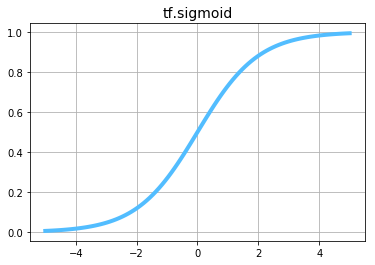
\includegraphics[width=0.65\textwidth]{./sync_imgs/act/smooth/sigmoid.png}
\label{fig:act_smooth_sigmoid}
\end{figure}

% {{{act_smooth_tangent}}}
\begin{figure}
\centering
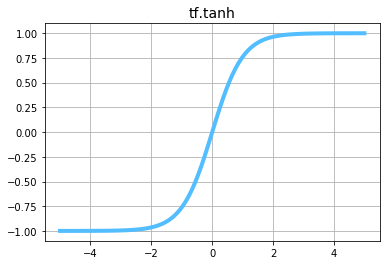
\includegraphics[width=0.65\textwidth]{./sync_imgs/act/smooth/tangent.png}
\label{fig:act_smooth_tangent}
\end{figure}

\subparagraph{ELU}

\textcolor{blue}{\textcolor{red}{CITE}. Smooth, monotonic, and non-zero in the negative portion of the input. The main drawback is that they are more computationally expensive (due to calculating the exponential)}


\begin{equation}
{
	ELU = f(x) = \left\{
	\begin{array}{ll}
	\alpha(e^x - 1) x & \quad $for$ \ x < 0 \\
	x & \quad $for$ \ x \ge 0
	\end{array}
	\right.
}
\label{eq:act_elu_def}
\end{equation}


% {{{act_smooth_elu}}}
\begin{figure}
\centering
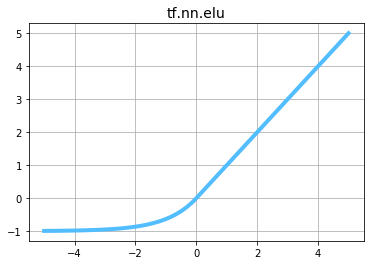
\includegraphics[width=0.65\textwidth]{./sync_imgs/act/smooth/elu.png}
\label{fig:act_smooth_elu}
\end{figure}

% {{{act_smooth_selu}}}
\begin{figure}
\centering
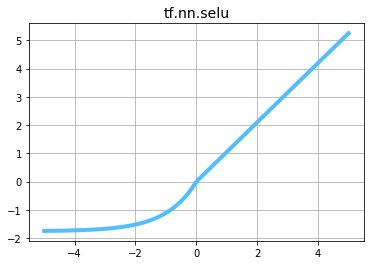
\includegraphics[width=0.65\textwidth]{./sync_imgs/act/smooth/selu.png}
\label{fig:act_smooth_selu}
\end{figure}


\subparagraph{Softplus}

\textcolor{blue}{continuous and differentiable at zero. However, due to the natural log and exponential function, there is added computation compared to th ReLU.}

% typcially discouraged in practice since ReLU achieves similar results and is less computationally expensive

\begin{equation}
{
	Softplus = f(x) = \ln{(1+e^x)}
}
\label{eq:act_softplus_def}
\end{equation}


% {{{act_smooth_softplus}}}
\begin{figure}
\centering
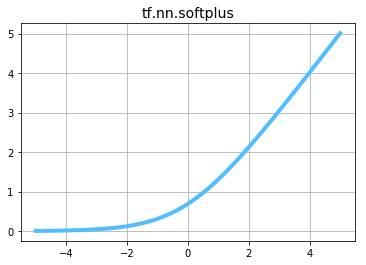
\includegraphics[width=0.65\textwidth]{./sync_imgs/act/smooth/softplus.png}
\label{fig:act_smooth_softplus}
\end{figure}

% {{{act_smooth_softsign}}}
\begin{figure}
\centering
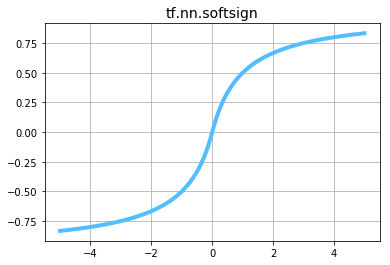
\includegraphics[width=0.65\textwidth]{./sync_imgs/act/smooth/softsign.png}
\label{fig:act_smooth_softsign}
\end{figure}


\paragraph{Not Smooth Non-linear}

\subparagraph{ReLU}

\begin{equation}
{
	ReLU = f(x) = \left\{
	\begin{array}{ll}
	0 & \quad $for$ \ x < 0 \\
	x & \quad $for$ \ x \ge 0
	\end{array}
	\right.
}
\label{eq:act_relu_def}
\end{equation}

% {{{act_notsmooth_relu}}}
\begin{figure}
\centering
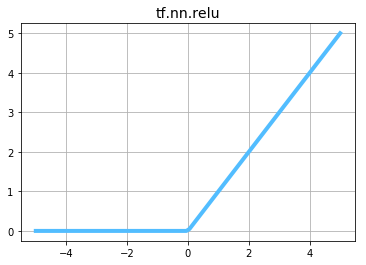
\includegraphics[width=0.65\textwidth]{./sync_imgs/act/notsmooth/relu.png}
\label{fig:act_notsmooth_relu}
\end{figure}

\subparagraph{Leaky ReLU}

\textcolor{blue}{The Leaky ReLU (Eq~\ref{eq:act_leaky_relu_def}) was designed in attempt to address the dying ReLU issue \textcolor{red}{CITE}. Rather than simply outputting a zero in the negative range, the Leaky ReLU will will have a small non-zero slope (user specified) -- allowing weight updating and training to continue.}

\textcolor{green}{TODO: randomized Leaky ReLU \textcolor{red}{cite} --- $\alpha$ (from PReLU) is sampled from a uniform distribution randomly. The net-effect could be considered similar to drop out since, technically, there is a different network for each value of $\alpha$, resulting in an ensemble of sorts. At test time, the values for $\alpha$ are averaged.}

\begin{equ}[!ht]
	\begin{equation}
	{
		Leaky ReLU = f(x) = \left\{
		\begin{array}{ll}
		N x & \quad $for$ \ x < 0 \\
		x & \quad $for$ \ x \ge 0
		\end{array}
		\right.
	}
	\label{eq:act_leaky_relu_def}
	\end{equation}
\caption{where $N$ is a constant. $N$ is typically set to 0.01}
\end{equ}

% {{{act_notsmooth_leakyrelu}}}
\begin{figure}
\centering
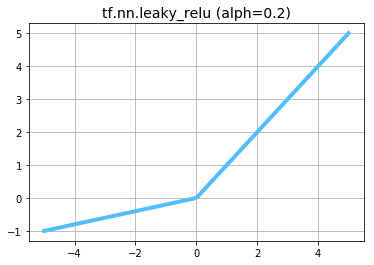
\includegraphics[width=0.65\textwidth]{./sync_imgs/act/notsmooth/leakyrelu.png}
\label{fig:act_notsmooth_leakyrelu}
\end{figure}

\subparagraph{ReLU6}

\textcolor{blue}{In general, this function is referred to as a {ReLUN}\index{ReLUN} function, where $N$ is some constant. However, in practice, $6$, was determined to be the optimal value.\textcolor{red}{CITE}. \textcolor{red}{This capped value, may help learn the sparse values sooner.} By having the upper limit bounded, the prepare the network for a fixed point precision for inference --- if the upper limit is unbounded, then you may loose too many bits to \textcolor{red}{Q} portion of the fixed point number.}
		

\textcolor{blue}{Similar to the ReLU fuction, only the output is capped to six in the positive domain.}

\begin{equation}
{
	ReLU6 = f(x) = min{(max{(0,x)},6)}
}
\label{eq:act_ReLU6_def}
\end{equation}

% {{{act_notsmooth_relu6}}}
\begin{figure}
\centering
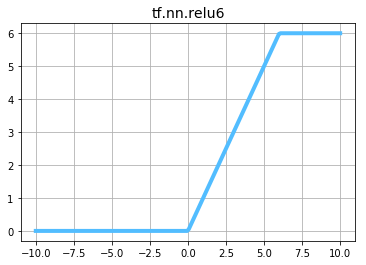
\includegraphics[width=0.65\textwidth]{./sync_imgs/act/notsmooth/relu6.png}
\label{fig:act_notsmooth_relu6}
\end{figure}

\subparagraph{PReLU}

\begin{equ}[!ht]
	\begin{equation}
	{
	PReLU = f(x) = \left\{
		\begin{array}{ll}
			\alpha x & \quad $for$ \ x < 0 \\
			x & \quad $for$ \ x \ge 0
		\end{array}
		\right.
	}
	\label{eq:act_prelu_def}
	\end{equation}
\caption{where $\alpha$ is a parameterized --- a learned parameter from training.}
\end{equ}

\textcolor{blue}{$\alpha$, rather than being hard coded, is determined during training by the data. The logic being that the value would be more optimal than we could set \textcolor{red}{CITE}}

% {{{act_notsmooth_prelu}}}
\begin{figure}
\centering
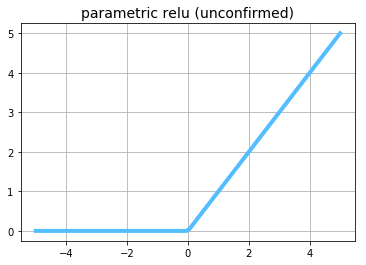
\includegraphics[width=0.65\textwidth]{./sync_imgs/act/notsmooth/prelu.png}
\label{fig:act_notsmooth_prelu}
\end{figure}




\section{Fine-Tuning Architectures}

\subsection{Profiler}

\subsection{Debugger}

\section{Distributed Training}
%% Section
\textcolor{blue}{see \textcolor{red}{local ref} for more detailed information about distributed training/evaluation.}


\subsection{Resource Management (GPU RAM)}
% TODO: implementation

\textcolor{blue}{By default, TensorFlow will allocate, and hold, all available GPU resources. This means if using \code{/GPU:0}, that 100\% of the resources will be dedicated to this program and so another tensorflow program cannot access this resource. Additionally, this means that if there are multiple GPU devices 100\% of those devices will also be allocated. If attempting to run two programs on the same device, with default settings, the following error will likely be encountered \code{CUDA\_ERROR\_OUT\_OF\_MEMORY}. This behavior can be controlled by either setting the device visibility or setting a device allocation threshold}

\paragraph{Device Visibility}

\textcolor{blue}{The environment variable \code{CUDA\_VISIBLE\_DEVICES} can be set to define specific device access for a program. e.g. \code{CUDA\_VISIBLE\_DEVICES=0,1} would allow the program access to only GPU devices 1 and 2.  Another program could then be started with \code{CUDA\_VISIBLE\_DEVICES=2,3} that would restrict it's access to GPUs 3 and 4}
\textcolor{blue}{For Example, if we only wanted the 3rd GPU to be accessed by a specific program, we could do the following (remember 0 based indexing):}

\begin{lstlisting}[style=pyInStyle]
import os
...
os.environ['CUDA_VISIBLE_DEVICES'] = '2'
\end{lstlisting}



\paragraph{Device Allocation}

\textcolor{blue}{It is also possible to only allow access to a specified fraction of a device i.e. n\% of a GPU.  This can be managed by altering the \code{ConfigProto} object. The \code{ConfigProto} object contains, among other configuration defaults (as messages), a message called \code{GPUOptions}. When running a session, these defaults can be changed. Within \code{GPUOptions}, there is a variable \code{per\_process\_gpu\_memory\_fraction} that is responsible for allocating a fraction of GPU memory.}

\textcolor{blue}{For example, if we wish to only allocate 40\% of a GPUs memory, we could do the following:}

\begin{lstlisting}[style=pyInStyle]
myConfig = tf.ConfigProto()
myConfig.gpu_options.per_process_gpu_memory_fraction = 0.4
session = tf.Session(config=myConfig)
\end{lstlisting}


\subparagraph{Allow Growth}

\textcolor{blue}{There is another option when managing the device memory. Rather than set a hard threshold, it is possible to allow TensorFlow to only allocate as much memory as it needs. This can be done by setting the \code{allow\_growth} bool to \code{True}. However, use caution with this option! \textbf{Once TensorFlow allocates memory, it is never released \textcolor{red}{``to avoid memory fragmentation''} i.e. running out of memory later is possible}}

\begin{lstlisting}[style=pyInStyle]
myConfig = tf.ConfigProto()
myConfig.gpu_options.allow_growth = True
session = tf.Session(config=myConfig)
\end{lstlisting}


\subsection{Device Placement}

\textcolor{blue}{A \textit{dynamic placer} algorithm is presented in the {TensorFlow whitepaper}~\cite{abadi2016tensorflow_device_placement} that is capable of automatically distributing operations across devices. This algorithm takes into consideration  estimates of the sizes of input and output tensors, computation time for each node, \textcolor{green}{OTHERS - TODO:read entire paper}.}

\textcolor{blue}{There is another (manual) placer called a \textit{simple placer}.}

% TODO: MORE...

% TODO: implementation



\section{Model Evaluation}

\textcolor{green}{TODO: para about using metrics.}

\textcolor{green}{Para about using tensorboard during training and tfma after training}

\textcolor{blue}{Metrics computed during training (e.g. training and validation metrics) can be visualized in tensorboard. Tensorboard displays, and continuously updates during training, these metrics graphically against global training steps (or time) and is used to determine how well your model is being trained. TFMA computes and visualizes metrics from the final (presumably after training) model. These metrics are computed only once. \textcolor{red}{TFMA exports and computes the metrics once on a saved model which contains the eval graph and additional metadata}}

\textcolor{blue}{Where tensorboard will compare models to each other over time, TFMA will compare models at only one point in time. This is better displayed in \textcolor{red}{see figure xx}.}

\textcolor{green}{TODO: figure showing the difference between graphs from tensorboard and TFMA}

\subsection{Metrics}

\textcolor{green}{TODO: talk about metrics/streaming metrics -- mention contrib}

\subsection{TensorBoard}

\subsection{TFMA: TensorFlow Model Analysis}


\section{Model Persistence}

\subsection{Saver}

\subsection{Hub}


%%%%%%%%%%%% Serving
\subsection{Serving}


\section{Other}

\subsection{Probability}

\subsection{TensorFlow Extended}

\subsection{Keras}

\subsection{Image}

\subsection{Image Augmentation}

\subsection{Edward 2.0}

\subsection{TensorFlow Lite}
